\documentclass[12pt,oneside,a4paper]{article}

\title{\textbf{Solar Tracker}}
\author{Enrico Sgarbanti - VR446095}

\usepackage{graphicx}
\usepackage{wrapfig}
% \usepackage{url}
\usepackage{hyperref}
\usepackage[italian]{babel}
\usepackage[utf8]{inputenc}

\begin{document}
\maketitle


\begin{abstract}
    Questo documento mostra la realizzazione di un semplice inseguitore solare ad un asse a scopo didattico realizzato con semplici componenti e un Arduino Nano.
\end{abstract}


\section{Introduzione}
L'obiettivo è la realizzazione di un dispositivo che sia in grado di ruotare rispetto ad un asse in modo da mostrare sempre la stessa faccia nel punto con più luce.


\section{Background}
Per la creazione di tale dispositivo sono state utilizzate varie competenze:


\subsection{Fotoresistenze}
\begin{figure}[!htb]
    \minipage{0.32\textwidth}
    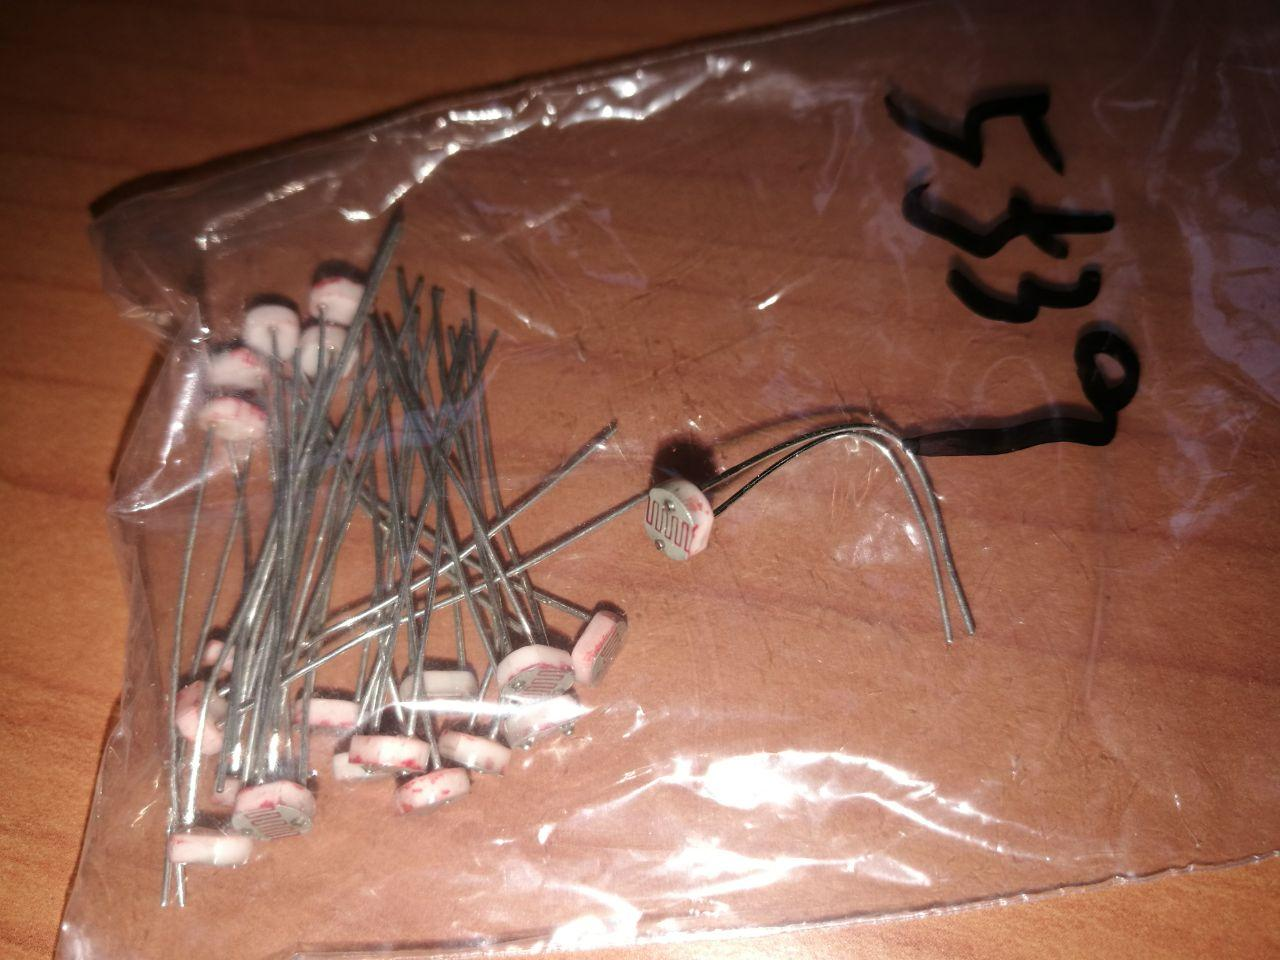
\includegraphics[width=\linewidth]{figures/fotoresistenze.jpg}
    \caption{Sacchetto di fotoresistenze.}
    \endminipage\hfill
    \minipage{0.32\textwidth}
    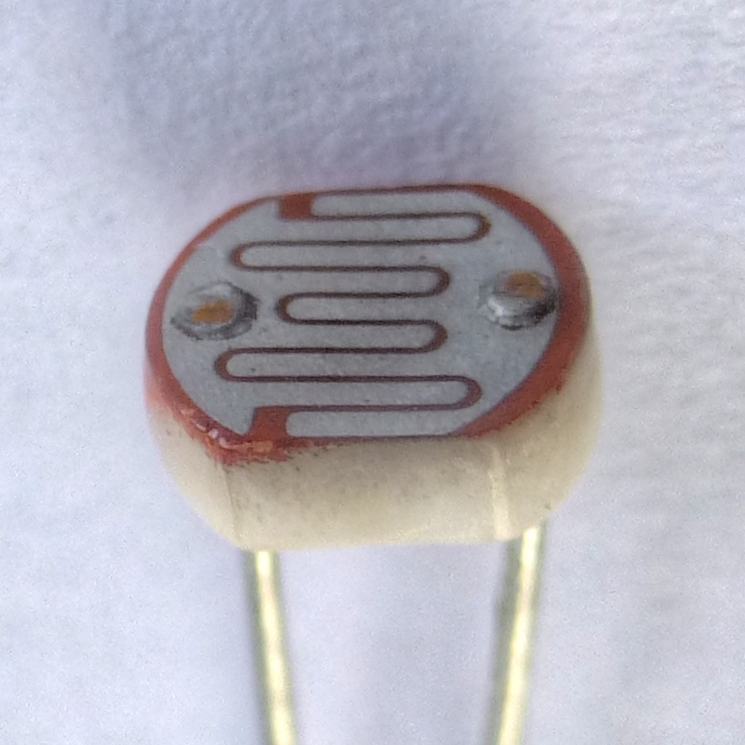
\includegraphics[width=\linewidth]{figures/fotoresistenza.jpg}
    \caption{Fotoresistenza}
    \endminipage\hfill
\end{figure}


\subsubsection{Introduzione}
Le fotoresistenze\cite{Photoresistor1}\cite{Photoresistor2}\cite{Photoresistor3} sono un componente elettronico la cui resistenza è inversamente proporzionale alla quantità di luce che lo colpisce, mentre la corrente elettrica che transita attraverso tale componente è proporzionale all'intensità di una sorgente luminosa.
\\Sebbene per la loro realizzazione venga utilizzato un materiale semiconduttore, essi sono dispositivi puramente passivi perché non possiedono una giunzione PN, e questo li separa da altri fotorilevatori come fotodiodi e fototransistori.


\subsubsection{Funzionamento}
I concetti alla base del funzionamento sono:
\begin{itemize}
    \item Una corrente elettrica consiste nel movimento di elettroni all'interno di un materiale.
    \item I buoni conduttori hanno un gran numero di elettroni liberi che possono spostarsi in una data direzione sotto l'azione di una differenza di potenziale.
    \item Gli isolanti ad alta resistenza hanno pochissimi elettroni liberi, quindi è difficile farli muovere cioè far scorrere una corrente.
    \item Una fotoresistenza è realizzata con del materiale semiconduttore ad alta resistenza, dovuta al fatto che ci sono pochissimi elettroni liberi di muoversi (la stragrande maggioranza degli elettroni è bloccata nel reticolo cristallino e incapace di muoversi).
\end{itemize}

\begin{figure}[!htb]
    \centering
    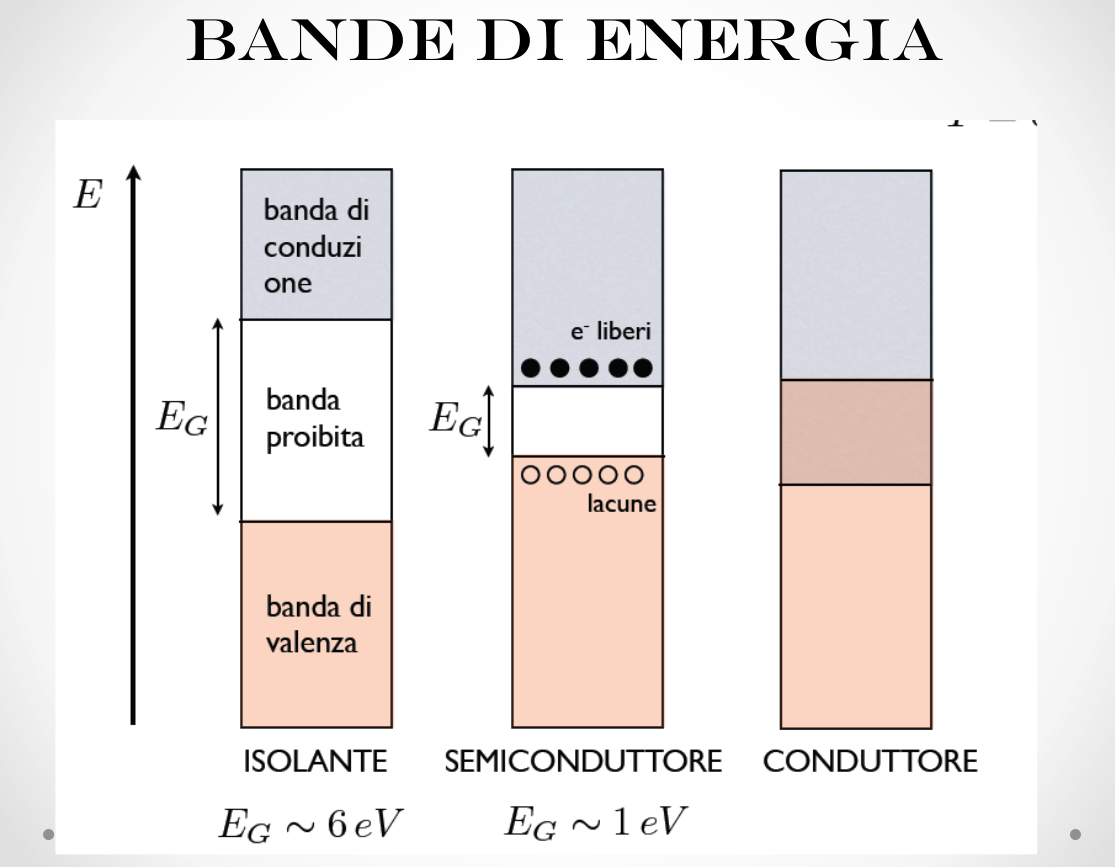
\includegraphics[width=0.45\linewidth]{figures/bande-energia.png}
    \caption{Bande di energia.}
\end{figure}

Quando la luce colpisce la fotoresistenza i fotoni vengono assorbiti dal reticolo del semiconduttore fornendo agli elettroni legati abbastanza energia da saltare nella banda di conduzione. Gli elettroni liberi risultanti (e le rispettive lacune) permettono lo scorrimento di corrente, riducendo di conseguenza la resistenza (effetto fotoconduttivo). Quando la luce incidente viene interrotta i portatori di carica in eccesso si ricombinano riportando la conducibilità del semiconduttore al suo valore iniziale in condizioni di oscurità.


\subsubsection{Struttura}
\begin{figure}[!htb]
    \minipage{0.5\textwidth}
    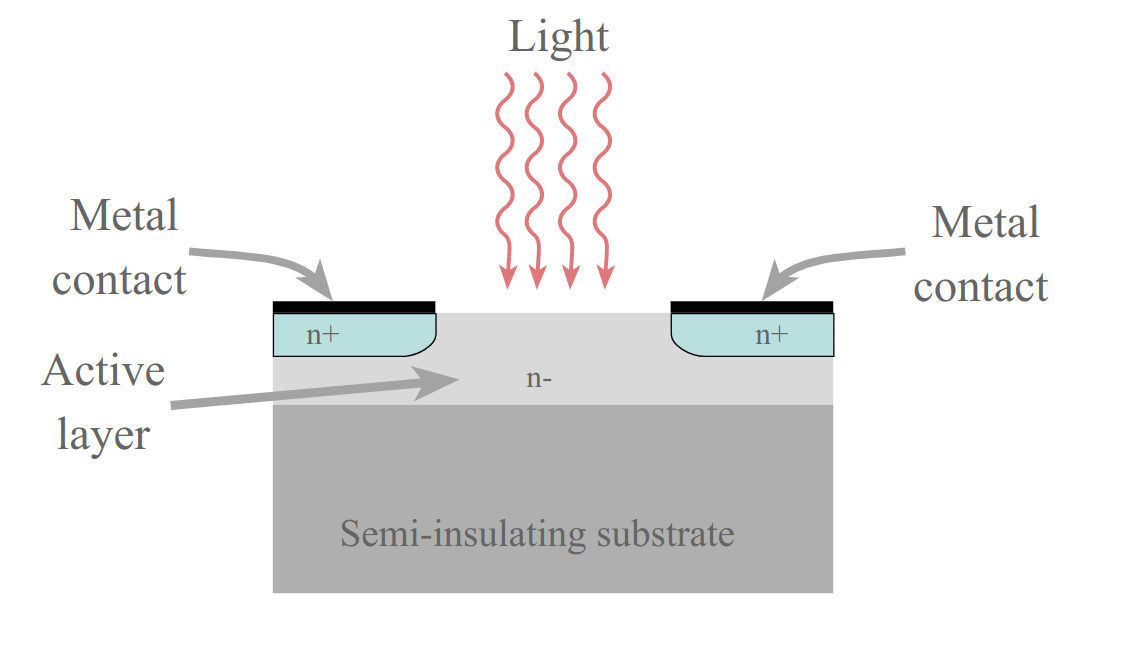
\includegraphics[width=\linewidth]{figures/fotoresistenza-struttura1.png}
    \caption{Struttura fotoresistenza.}
    \endminipage\hfill
    \minipage{0.5\textwidth}
    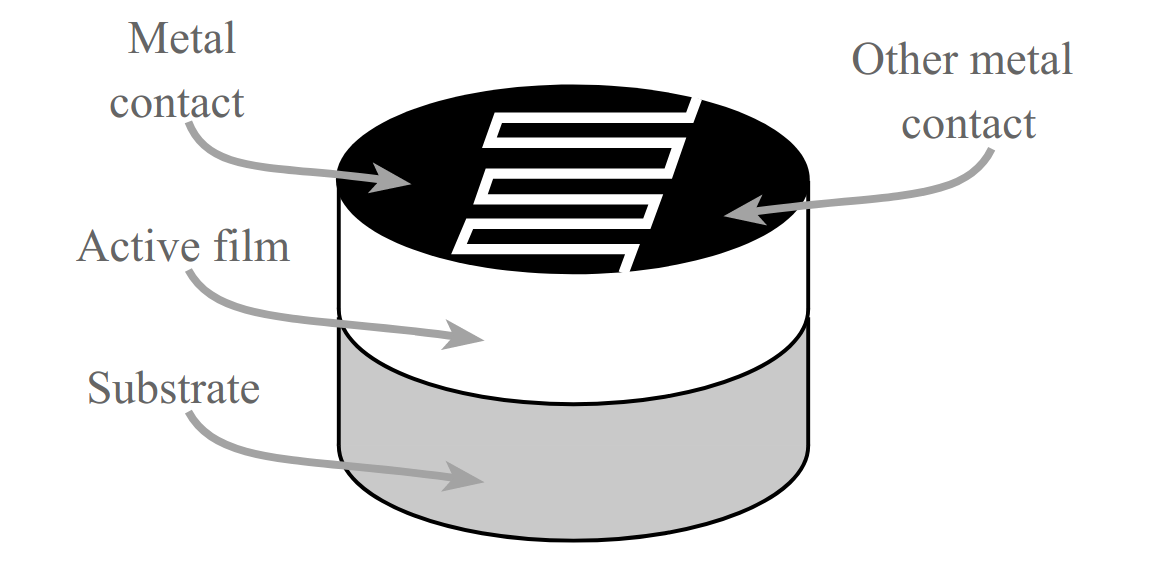
\includegraphics[width=\linewidth]{figures/fotoresistenza-struttura2.png}
    \caption{Struttura fotoresistenza.}
    \endminipage\hfill
\end{figure}

Normalmente la fotoresistenza è formata da un substrato semiisolante, sul quale è depositato il semiconduttore (solitamente leggermente drogato). Sopra di esso vi è posta una superficie metallica la quale è però divisa a metà dal semiconduttore con un ''interdigital pattern`` per aumentare l'area esposta alla luce.
\\I semiconduttori tipicamente usati sono CdSe, CdS, CdTe, InSb, InP, PbS, PbSe, Ge, Is, GaAs. Ogni materiale offre proprietà diverse in termini di lunghezza d'onda, della sensibilità, ...
\\Si parla di \textbf{fotoresistenze intrinseche} quando vengono utilizzano materiali semiconduttori non drogati tra cui silicio o germanio. I fotoni cadono sugli elettroni di eccitazione spostandoli dalla banda di valenza alla banda di conduzione. Di conseguenza, questi elettroni sono liberi di condurre l'elettricità.
\\Più luce cade sul dispositivo, più elettroni vengono liberati, maggiore è il livello di conduttività, e minore sarà il livello di resistenza.
\\Si parla invece di \textbf{fotoresistenze estrinseche} quando vengono utilizzati materiali semiconduttori drogati con impurità. Queste impurità creano una nuova banda di energia sopra la banda di valenza esistente. Di conseguenza, gli elettroni hanno bisogno di meno energia per trasferirsi nella banda di conduzione.


\subsubsection{Dipendenza dalla frequenza}
\begin{figure}[!htb]
    \centering
    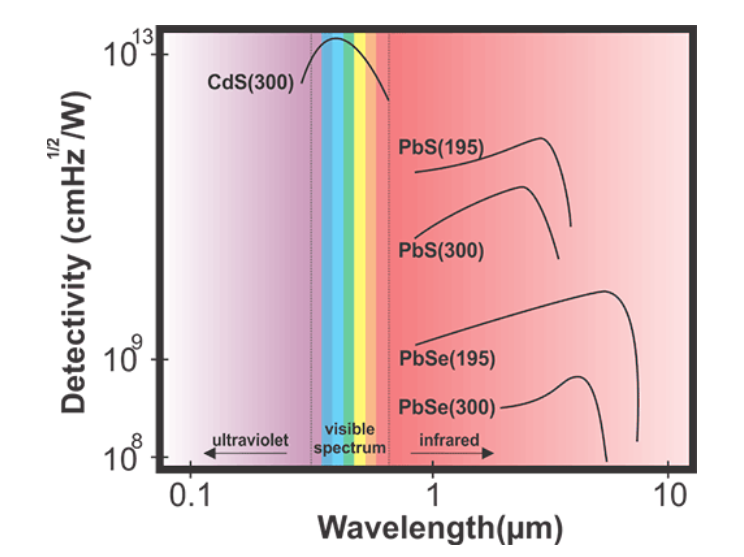
\includegraphics[width=0.6\linewidth]{figures/frequenza.png}
    \caption{Lunghezze d'onda.}
\end{figure}
In base al materiale utilizzato le fotoresistenze reagiscono in modo diverso alla luce di diverse lunghezze d'onda.
\\Le fotoresistenze estrinseche tendono ad essere più sensibili alla luce a lunghezza d'onda più lunga e possono essere usati per gli infrarossi. Tuttavia, quando si lavora con gli infrarossi, è necessario prestare attenzione per evitare l'accumulo di calore causato.


\subsubsection{Latenza}
Un aspetto importante da tenere in considerazione è quello della latenza cioè il tempo impiegato dal componente per rispondere ad un qualsiasi cambiamento. La velocità con cui cambia la resistenza è chiamata \textbf{resistence recovery rate}.
\\ Normalmente la fotoresistenza risponde entro poche decine di millisecondi quando la luce viene applicata dopo l'oscurità totale, ma quando la luce viene rimossa può richiedere fino a un secondo circa affinché la resistenza raggiunga il suo livello finale. Per questo motivo la fotoresistenza non è una buona scelta dove ci sono valori di cambiamento ragionevolmente rapidi di luce. Tuttavia, quando i cambiamenti di luce avvengono per un periodo di tempo prolungato, sono più che adeguati.


\subsubsection{Applicazioni di fotoresistenza}
Essendo dispositivi semplici economici e robusti, le fotoresistenze sono utilizzate in diverse applicazioni. Alcuni esempi di applicazioni sono sistemi per il controllo dell'illuminazione, lampioni, allarmi antifurto, raiosveglie, esposimetri, ...


\subsection{Partitore di tensione}
\begin{figure}[!htb]
    \centering
    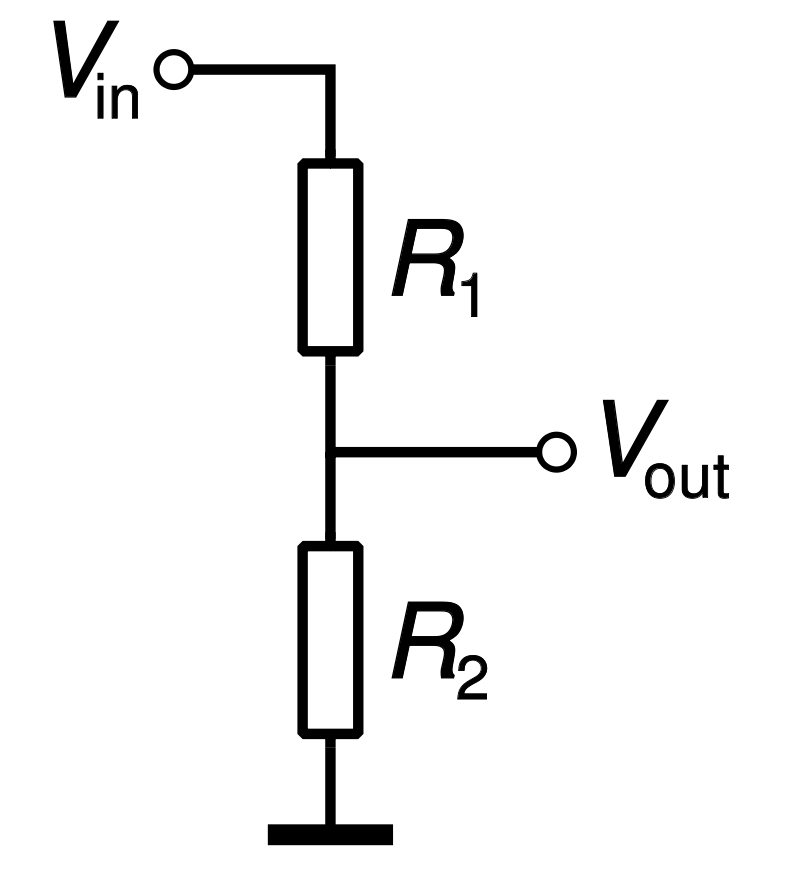
\includegraphics[width=0.3\linewidth]{figures/partitore_tensione.png}
    \caption{Partitore di tensione.}
\end{figure}
Il partitore di tensione\cite{VoltageDivider} è un tipo di circuito costituito da due o più componenti passivi collegati in serie ai capi dei quali, se viene applicata una tensione, essa si ripartirà sulle stesse componenti in base al loro valore.
Grazie all'applicazione della legge di Ohm e della legge di Kirchhoff si ricava che $V_{out} = V_{in} \frac{R_2}{R_1 + R_2}$.
\\Dalla formula si può notare che:
\begin{itemize}
    \item $V_{out} = \frac{V_{in}}{2}$ se $R_1 = R_2$.
    \item $V_{out} > \frac{V_{in}}{2}$ se $R_1 < R_2$.
    \item $V_{out} < \frac{V_{in}}{2}$ se $R_1 > R_2$.
\end{itemize}


\subsection{Motore passo-passo 4-fasi unipolare}

\begin{figure}[!htb]
    \centering
    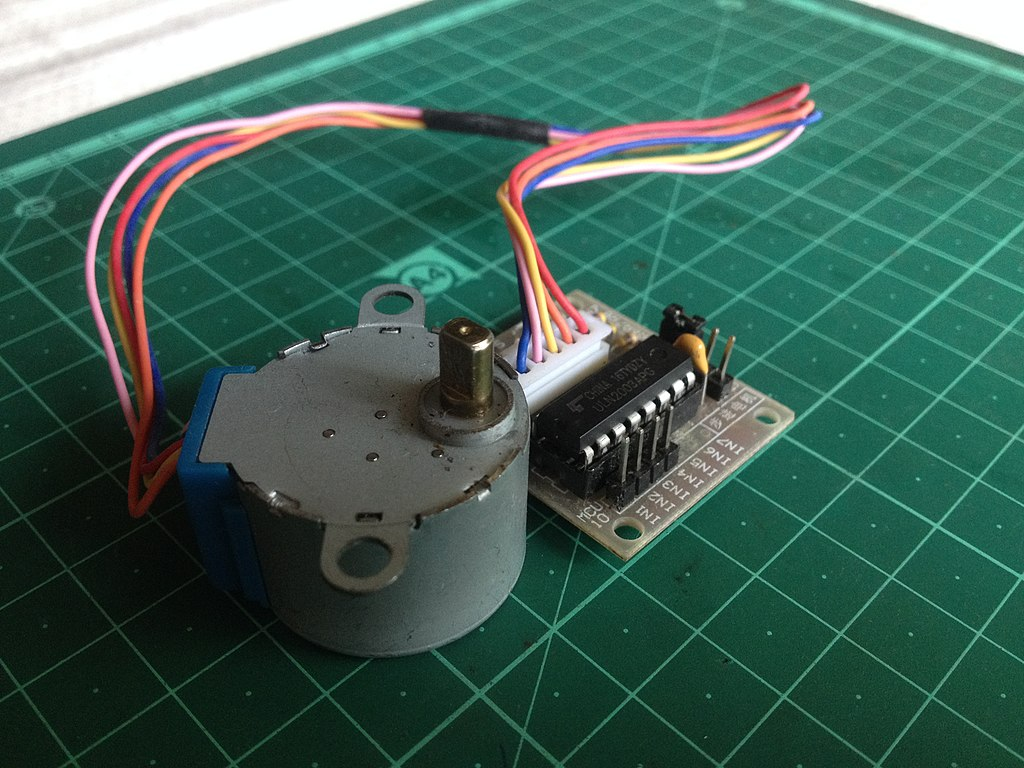
\includegraphics[width=0.4\linewidth]{figures/motor28BYJ-48.jpg}
    \caption{Motore 28BYJ-48.}
\end{figure}
Un motore passo-passo\cite{StepMotor} è un motore DC brushless che divide una rotazione completa in un numero di passi uguali.
A differenza degli altri motori, ha come scopo quello di mantenere fermo il rotore in una posizione di equilibrio: se alimentato si limita infatti a bloccarsi in una ben precisa posizione angolare. Per farlo muovere bisogna quindi inviare una serie di impulsi di corrente in un'opportuna sequenza.
\\È quindi possibile far muovere il rotore nella posizione e alla velocità voluta semplicemente contando gli impulsi ed impostando la loro frequenza, visto che le posizioni di equilibrio del rotore sono determinate meccanicamente con estrema precisione.

\begin{figure}[!htb]
    \centering
    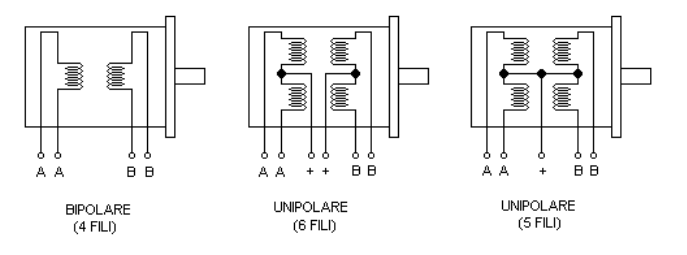
\includegraphics[width=0.8\linewidth]{figures/unipolare-bipolare.png}
    \caption{Struttura motori unipolari e bipolari.}
\end{figure}

I motori unipolari, a differenza di quelli bipolari, hanno uno o due fili in più che portano l'alimentazione e non necessitano di invertire la polarità sulle fasi.

\begin{figure}[ht!]
    \centering
    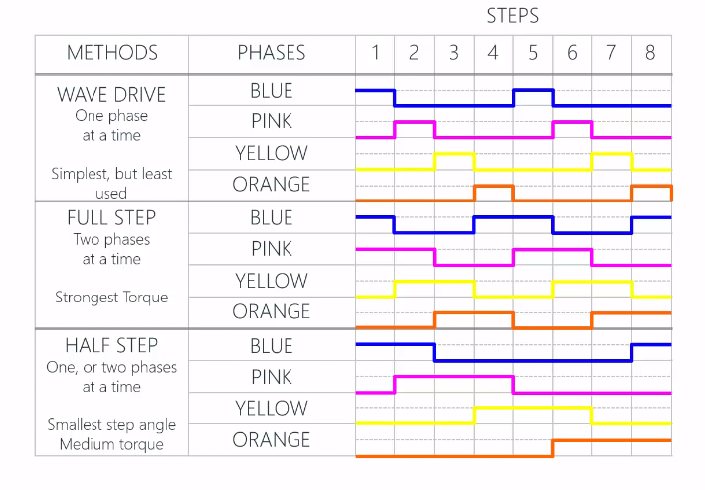
\includegraphics[width=0.8\textwidth]{figures/motor-sequence.png}
    \caption{Sequenza impulsi motore.}
\end{figure}
Un motore passo-passo è idealmente guidato da corrente sinusoidale. Sono state sviluppate varie tecniche di azionamento per approssimare meglio una forma d'onda di azionamento sinusoidale:
\begin{itemize}
    \item \textbf{Wave drive (una fase attivata): } Viene attiva una sola fase alla volta. Ha lo stesso numero di step dell'azionamento full-step, ma il motore avrà una coppia significativamente inferiore a quella nominale. È molto semplice, ma è usato raramente
    \item \textbf{Full-step drive (due fasi attive): } Sono sempre attive due fasi in modo che il motore fornisca la massima coppia nominale. Non appena viene disattivata una fase, ne viene attivata un'altra. Richiede più corrente, ma fornisce il doppio della coppia.
    \item \textbf{Half-stepping: } Si alterna tra una e due fasi. Viene attivata una fase, nel ciclo successivo un altra e in quello dopo ancora viene disattivata la prima. Richiede più corrente, ma fornisce una miglior precisione.
\end{itemize}


\subsection{Arduino}
\begin{figure}[!htb]
    \centering
    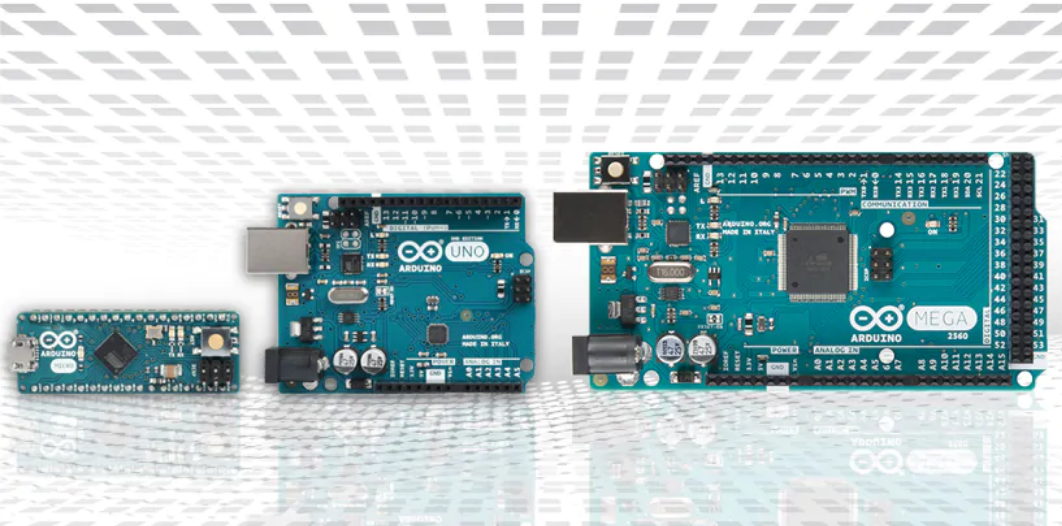
\includegraphics[width=0.5\linewidth]{figures/arduino.png}
    \caption{Schede Arduino Nano, Arduino UNO, Arduino Mega.}
\end{figure}
Arduino\cite{Arduino} è una piattaforma elettronica open source basata su hardware e software di facile utilizzo. Le schede Arduino permettono di leggere input da sensori, elaboratore i dati nel microcontrollore programmabile e restituire output mediante attuatori

\clearpage
\begin{figure}[!htb]
    \centering
    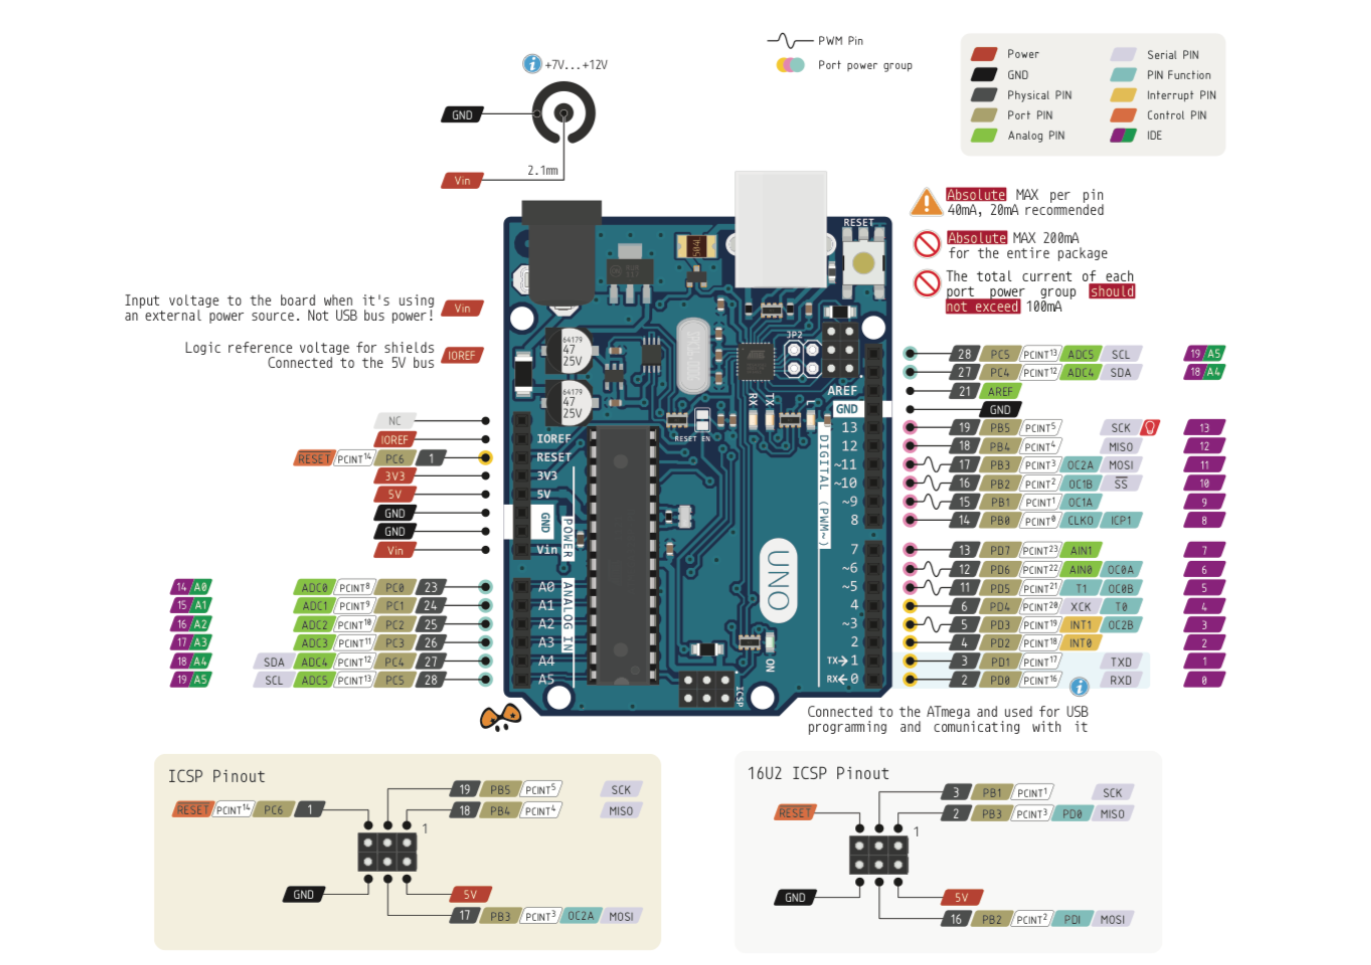
\includegraphics[width=0.90\linewidth]{figures/arduinoUNO.png}
    \caption{Arduino UNO.}
\end{figure}

\begin{figure}[!htb]
    \centering
    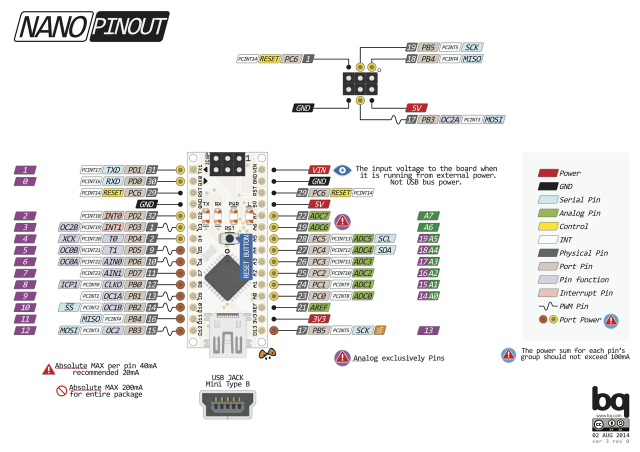
\includegraphics[width=0.90\linewidth]{figures/arduinoNANO.png}
    \caption{Arduino Nano.}
\end{figure}
Arduino è nato all'Ivrea Interaction Design Institute come uno strumento semplice per la prototipazione rapida, rivolto a studenti senza esperienza in elettronica e programmazione. Non appena ha raggiunto una comunità più ampia, la scheda Arduino ha iniziato a cambiare per adattarsi alle nuove esigenze e sfide, differenziando la sua offerta da semplici schede a 8 bit a prodotti per applicazioni IoT, indossabili, stampa 3D e ambienti incorporati. Tutte le schede Arduino sono completamente open-source, consentendo agli utenti di costruirle in modo indipendente e alla fine adattarle alle loro esigenze particolari. Anche il software è open source e sta crescendo grazie al contributo degli utenti di tutto il mondo.


\section{Solar Tracker}

\subsection{Struttura e componenti}
Il dispositivo è stato realizzato con:
\begin{itemize}
    \item 1x Arduino NANO
    \item 1x Stepper motor 28BYJ-48 \cite{MotorDatasheet}
    \item 1x Driver board ULN2003 \cite{DriverMotorDatasheet}
    \item 2x Photoresistor GL5537
\end{itemize}


\begin{figure}[!htb]
    \centering
    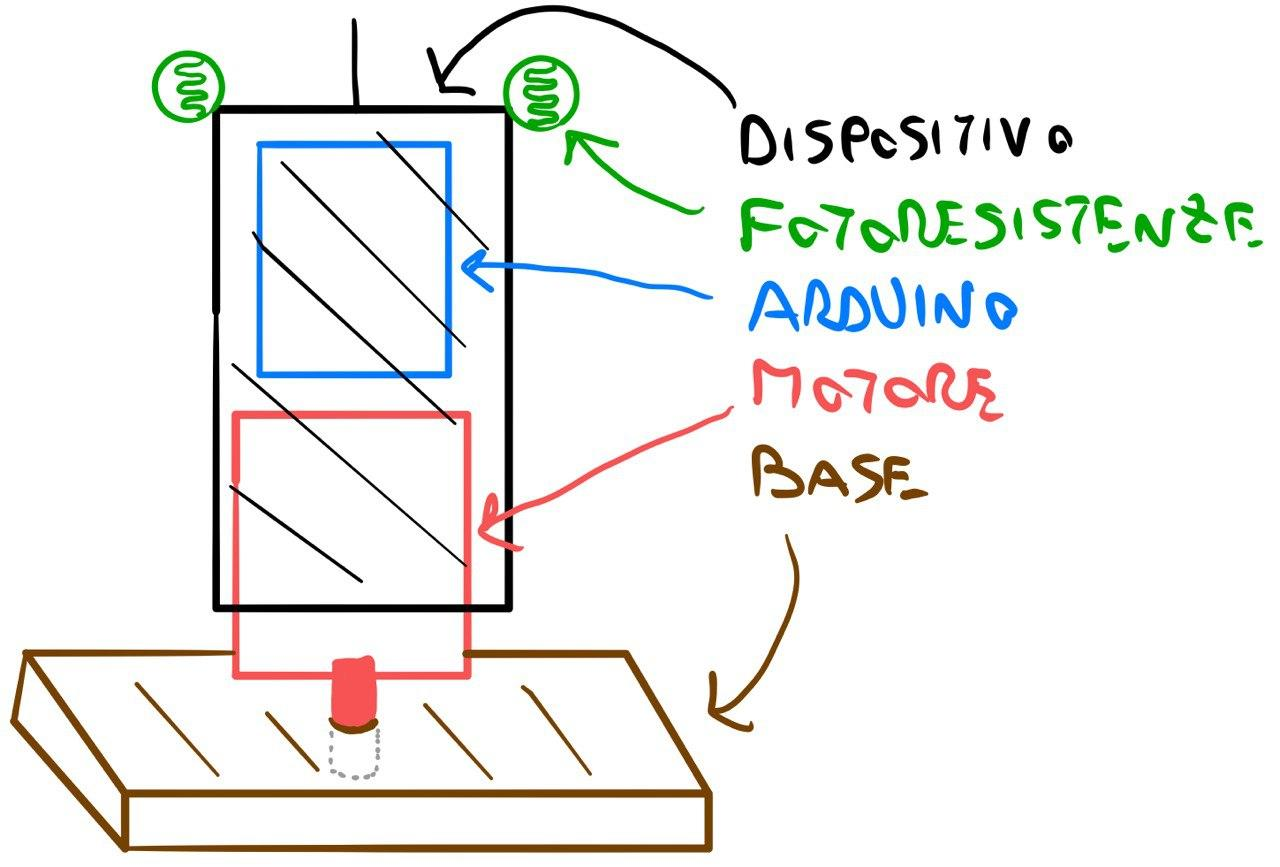
\includegraphics[width=0.5\linewidth]{figures/modello_solar_tracker}
    \caption{Struttura esemplificativa.}
\end{figure}
Al fine di permettere la completa rotazione, impossibile altrimenti a causa dei cavi, tutti i componenti sono stati disposti all'interno di una scatola tranne le fotoresistenze che si trovano nella parte superiore separate da un divisorio. (Il motore utilizzato non è il più adatto per questa scelta, ma essendo un prototipo a scopo didattico è stato utilizzato quello già visto a lezione)

\subsection{Funzionamento}
Ad un intervallo fissato l'Arduino inizierà a leggere il voltaggio generato dal partitore di tensione con le due fotoresistenze per far muovere il motore fino a raggiungere la posizione di equilibrio ovvero quella in cui nella faccia del dispositivo è presente più luce.
L'intervallo fissato dipenderà dal tipo di applicazione, per esempio se lo scopo fosse quello di disporre un pannello solare sempre verso il sole allora sarebbe inutilmente dispendioso azionare l'Arduino ogni 10 secondi.

\subsubsection{Fotoresistenze}

\begin{figure}[!htb]
    \centering
    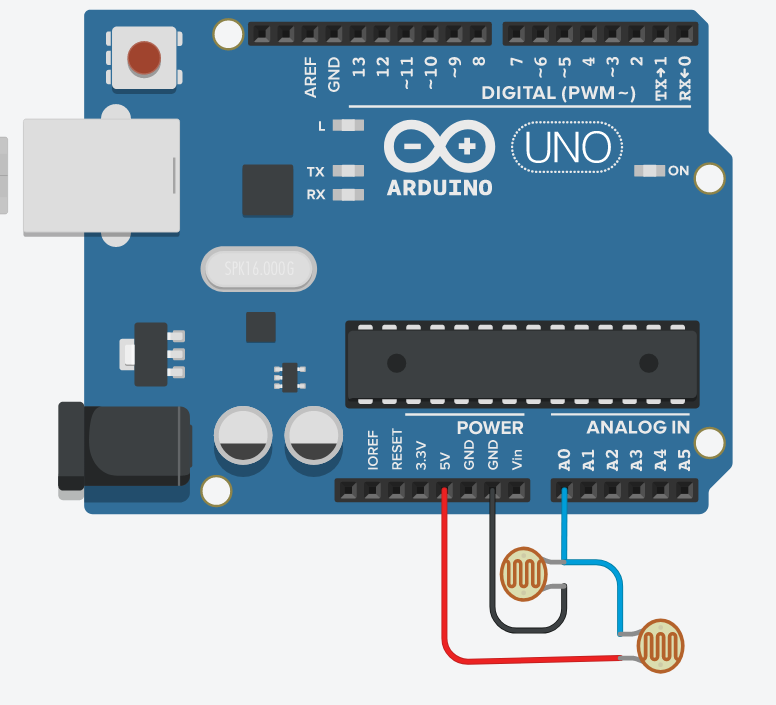
\includegraphics[width=0.4\linewidth]{figures/photoresistors}
    \caption{Collegamento fotoresistenze ad un Arduino UNO.}
\end{figure}
Grazie a due fotoresistenze dello stesso tipo è possibile trovare il punto in cui c'è più luce, ovvero quello in cui faranno la stessa resistenza.
\\Per fare ciò bisogna inserirle in un partitore di tensione collegato ad un AnalogInput dell'Arduino e leggere il valore di tensione:
\begin{itemize}
    \item se la tensione è 2.5V (cioè la metà dei 5V passati al partitore) allora le due fotoresistenze stanno facendo la stessa resistenza e quindi stanno ricevendo la stessa quantità di luce. Perciò si è arrivati alla posizione desiderata.
    \item se la tensione è maggiore di 2.5V allora la fotoresistenza collegata direttamente ai 5V sta facendo meno resistenza rispetto alla seconda e quindi è quella che sta ricevendo più luce.
    \item se la tensione è minore di 2.5V allora la prima resistenza sta facendo più resistenza rispetto alla seconda e quindi è quella che sta ricevendo meno luce.
\end{itemize}

\subsection{Elaborazione inputs}
Durante la ricerca del punto di equilibrio il dispositivo ad ogni ciclo deve leggere il valore di tensione dato dal partitore di tensione e dire al motore in che direzione andare fino alla lettura del valore di 2.5V.
\\Essendo però difficile leggere esattamente il valore 2.500, il sistema risulterà instabile, continuando ad oscillare alla ricerca del punto di equilibrio.
\\Per risolvere questo problema basta fermare il motore non quando la tensione è uguale a 2.5V bensì quando è minore di $2.5 - |epsilon|$ Volt.
\\Un primo approccio vede epsilon come numero fisso, ma questo valore dipende da vari fattori e quindi risulta poco flessibile.
\\Un secondo approccio che supera queste limitazioni vede epsilon come numero variabile, che partendo da 0 cresce ogni volta che c'è una inversione di rotazione.


\subsection{Utilizzo del motore}
Il motore utilizzato è un motore passo-passo unipolare a 4 fasi che è collegato ad una driver board che permette di controllarlo facilmente alimentando i quattro input della board.
\\La tecnica utilizzata per l'avanzamento è la full-step, in quanto la più consigliata.


\subsection{Considerazioni}
Aggiungendo un altro motore è possibile estendere la ricerca della posa con più luce tenendo conto di tutte e 3 le dimensioni.
Grazie a questo miglioramento è possibile realizzare un dispositivo che permetta ad un pannello solare di essere posizionato sempre nella posizione che dia la maggior efficienza.


\bibliographystyle{ieeetr}
\bibliography{biblio}


\end{document}